\documentclass[russian,14pt,twoside]{extreport}
\usepackage[T2A]{fontenc}
\usepackage[utf8]{inputenc}
\usepackage[english,main=russian]{babel}
\usepackage{iflang}
%%----------------------------------------------------------------------------
\usepackage{setspace}
\selectfont
\parindent=18pt
\frenchspacing
%%----------------------------------------------------------------------------
\usepackage{amsmath}
\usepackage{amssymb}
\usepackage{amscd}
\usepackage{etoolbox}
\usepackage{mathtools}
\usepackage{bm}
\usepackage[labelformat=empty]{caption}
\usepackage{graphicx}
\usepackage[all]{xy}
\usepackage{url}
\usepackage{listings}
\usepackage{array}
\usepackage{tabularx}
\usepackage{booktabs}
%%----------------------------------------------------------------------------
\usepackage[%
        a4paper,%
        includehead,%
        left=2.3cm,%
        top=2.3cm,%
        right=2.3cm,%
        bottom=2.3cm,%
        headheight=0.7cm,%
        headsep=0.3cm,%
        footskip=1.6cm]{geometry}
\special{papersize=210mm,297mm}
%%----------------------------------------------------------------------------
\renewcommand{\thefootnote}{\fnsymbol{footnote}}
%%----------------------------------------------------------------------------
\usepackage{fancyhdr}
\pagestyle{fancy}%
\fancyhead{}%
\fancyfoot{}%
\fancyhead[LE,RO]{\normalsize \thepage}%
\fancyhead[RE,LO]{\leftmark}
%%----------------------------------------------------------------------------
\raggedbottom
%%----------------------------------------------------------------------------
\makeatletter
%%----------------------------------------------------------------------------
\protected\def\switchinitials#1{%
\begingroup%
\edef\temp{\endgroup%
    \noexpand\switchinitials@fixcomma%
    \forcsvlist{\switchinitials@item}{#1}\relax}%
    \temp}
\def\switchinitials@fixcomma, #1{#1}
\def\switchinitials@item#1{, \switchinitials@single#1\relax}
\def\switchinitials@single#1~#2\relax{#2~#1}
%%----------------------------------------------------------------------------
\newenvironment{ptkarticle}[3][russian]{%
\begin{otherlanguage}{#1}
\pagebreak[2]
\vskip 30pt plus 12pt minus 6pt
{\leftskip=1.5\parindent
\rightskip=1.5\parindent
\vbox{\centering\sffamily\bfseries\Large #2}}
\markboth{\switchinitials{#3}}{}
\nopagebreak
\vskip 6pt
\@afterheading
}{%
\end{otherlanguage}
}
%%----------------------------------------------------------------------------
\newcommand\OneAuthor[3]{%
\vbox{%
{\centering\bfseries\normalsize #1\par}
\vskip 3pt
\raggedright
\leavevmode\noindent\footnotesize
\hangindent=18pt\hangafter=1
#2, e-mail: \texttt{#3}\\*\par}
\nopagebreak
\medskip
\@afterheading
}
%%----------------------------------------------------------------------------
\newcommand\TwoAuthor[6]{%
\vbox{%
{\centering\bfseries\normalsize #1$^1$, #4$^2$\\}
\vskip 3pt
\raggedright
\leavevmode\noindent\footnotesize
\hangindent=18pt\hangafter=1
$^1$ {#2}, e-mail: \texttt{#3}\par
\hangindent=18pt\hangafter=1
$^2$ {#5}, e-mail: \texttt{#6}\\*\par}
\nopagebreak
\smallskip
\@afterheading
}
%%----------------------------------------------------------------------------
\newcommand\ThreeAuthor[9]{%
\vbox{%
{\centering\bfseries\normalsize #1$^1$, #4$^2$, #7$^3$\\}
\vskip 3pt
\raggedright
\leavevmode\noindent\footnotesize
\hangindent=18pt\hangafter=1
$^1$ {#2}, e-mail: \texttt{#3}\par
\hangindent=18pt\hangafter=1
$^2$ {#5}, e-mail: \texttt{#6}\par
\hangindent=18pt\hangafter=1
$^3$ {#8}, e-mail: \texttt{#9}\\*\par}
\nopagebreak
\smallskip
\@afterheading
}
%%----------------------------------------------------------------------------
\newcommand\FourAuthor[9]{%
\def\Argi{{#1}}%
\def\Argii{{#2}}%
\def\Argiii{{#3}}%
\def\Argiv{{#4}}%
\def\Argv{{#5}}%
\def\Argvi{{#6}}%
\def\Argvii{{#7}}%
\def\Argviii{{#8}}%
\def\Argix{{#9}}%
\FourAuthorContinue
}
\newcommand\FourAuthorContinue[3]{%
\vbox{%
{\centering
{\bfseries\normalsize \Argi$^1$, \Argiv$^2$, \Argvii$^3$, #1$^4$\\}}
\vskip 3pt
\raggedright
\leavevmode\noindent\footnotesize
\hangindent=18pt\hangafter=1
$^1$ \Argii, e-mail: \texttt{\Argiii}\par
\hangindent=18pt\hangafter=1
$^2$ \Argv, e-mail: \texttt{\Argvi}\par
\hangindent=18pt\hangafter=1
$^3$ \Argviii, e-mail: \texttt{\Argix}\par
\hangindent=18pt\hangafter=1
$^4$ #2, e-mail: \texttt{#3}\\*\par}
\nopagebreak
\smallskip
\@afterheading
}
%%----------------------------------------------------------------------------
\newcommand\FiveAuthor[9]{%
\def\Argi{{#1}}%
\def\Argii{{#2}}%
\def\Argiii{{#3}}%
\def\Argiv{{#4}}%
\def\Argv{{#5}}%
\def\Argvi{{#6}}%
\def\Argvii{{#7}}%
\def\Argviii{{#8}}%
\def\Argix{{#9}}%
\FiveAuthorContinue
}
\newcommand\FiveAuthorContinue[6]{%
\vbox{%
{\centering
\bfseries\normalsize \Argi$^1$, \Argiv$^2$, \Argvii$^3$, #1$^4$, #4$^5$\\}
\vskip 3pt
\raggedright
\leavevmode\noindent\footnotesize
\hangindent=18pt\hangafter=1
$^1$ {\Argii}, e-mail: \texttt{\Argiii}\par
\hangindent=18pt\hangafter=1
$^2$ {\Argv}, e-mail: \texttt{\Argvi}\par
\hangindent=18pt\hangafter=1
$^3$ {\Argviii}, e-mail: \texttt{\Argix}\par
\hangindent=18pt\hangafter=1
$^4$ {#2}, e-mail: \texttt{#3}\par
\hangindent=18pt\hangafter=1
$^5$ {#5}, e-mail: \texttt{#6}\\*\par}
\nopagebreak
\smallskip
\@afterheading
}
%%----------------------------------------------------------------------------
\newcommand\Subtitle[1]{
\medskip
\noindent
{\bfseries\large #1}
\par\nopagebreak
\smallskip
\@afterheading
}
%%----------------------------------------------------------------------------
\usepackage{enumitem}
\setlist[enumerate]{%
    %labelindent=0pt by default
    leftmargin=*,%
    topsep=4pt plus 2pt minus 2pt,%
    partopsep=2pt plus 1pt minus 1pt,%
    parsep=2pt plus 1pt,%
    itemsep=2pt plus 1pt%
}
\setlist[itemize]{%
    %labelindent=0pt by default
    leftmargin=*,%
    topsep=4pt plus 2pt minus 2pt,%
    partopsep=2pt plus 1pt minus 1pt,%
    parsep=2pt plus 1pt,%
    itemsep=2pt plus 1pt%
}
%%----------------------------------------------------------------------------
\newenvironment{ptkreferences}{
\pagebreak[1]
\medskip
\noindent
{\scshape\large \IfLanguageName{russian}{Список литературы}{References}}
\par\nopagebreak
\smallskip
\@afterheading
\begin{enumerate}[label={[\arabic*]},leftmargin=*]
}{
\end{enumerate}
}
%%----------------------------------------------------------------------------
\binoppenalty=10000
\relpenalty=10000
\@clubpenalty=10000
\clubpenalty=10000
\widowpenalty=10000
%%----------------------------------------------------------------------------
\defineshorthand[russian]{"*}{\mbox{-}\bbl@allowhyphens}
%%----------------------------------------------------------------------------
\makeatother
%%----------------------------------------------------------------------------
\begin{document}
\begin{ptkarticle}%
{Задачи обслуживания бинарного потока объектов в системе с двумя накопительно"=расходными компонентами}{Пудов~А.\,С.}
\OneAuthor%
{Пудов Андрей Семенович}%
    {Волжский государственный университет водного транспорта}{andrey@andreypudov.com}%

Рассматривается модель одностадийного обслуживания конечного детерминированного потока объектов процессором с накопительно"=расходным компонентом --- резервуаром ограниченной емкости. Поток состоит из подпотока объектов, пополняющих резервуар, и подпотока объектов, заполняемых из резервуара. С каждым объектом ассоциируется линейная функция индивидуального штрафа за время пребывания в системе обслуживания. Изучается задача построения расписания, минимизирующего суммарный штраф по всем объектам потока. Конструируемые алгоритмы основываются на принципе динамического программирования. Приводятся результаты вычислительных экспериментов.

{\itshape Ключевые слова:} расписание обслуживания, динамическое программирование, NP-трудность

% \Subtitle{Введение}

% Рассматриваемая модель возникла при изучении процессов грузовой обработки танкерного флота в условиях Северного завоза~[1] через речной порт г. Салехарда.

% В течение непродолжительного навигационного периода крупнотоннажным танкерным флотом по реке Обь с нефтеперегонных заводов Западной Сибири в Салехардский порт доставляется дизельное топливо. Прибывающие суда в определенной очередности подаются к специализированному терминалу, техническими средствами которого нефтепродукт перекачивается в резервуар ограниченной ёмкости. Многочисленные пункты потребления дизельного топлива, являющегося основным энергетическим ресурсом в Заполярье, располагаются, в основном, по берегам Обской губы и малых рек прилегающего региона полуострова Ямал. Доставка топлива в эти пункты осуществляется водным путем из Салехардского порта малотоннажными танкерами ледового класса, загрузка которых осуществляется на вышеупомянутом специализированном терминале; по техническим условиям на этом терминале не может одновременно обслуживаться более одного танкера.

% В описанной схеме Северного завоза задействованы танкеры, характеризующиеся различными технико-экономическими параметрами. Задача диспетчеризации заключается в выработке стратегии управления очередностью их грузовой обработки --- расписания обслуживания, которое в пределах горизонта оперативного планирования обеспечивает сокращение суммарных эксплуатационных расходов, обусловлен- ных непроизводительными простоями флота.

% Специфика задач диспетчеризации заключается в том, что между моментом, когда полностью определились исходные данные конкретной задачи, и моментом, когда следует начать работу по построенному расписанию, проходит относительно небольшой промежуток времени. В течение этого промежутка задача должна быть решена. Поэтому при математическом исследовании каждой типовой задачи диспетчеризации важно получить оценку ее вычислительной сложности. Вячеслав Сергеевич Танаев был одним из первых математиков, активно исследовавших вопросы вычислительной сложности задач теории расписаний; в написанных им совместно с коллегами и получивших мировое признание монографиях~[2,\,3,\,4] вопросы разделения задач на полиномиально разрешимые и NP-трудные~[5] играют ключевую роль.

% Статья состоит из шести разделов и Приложения. В следующем за Введением разделе 2 приводится описание модели обслуживания, дана математическая постановка задачи синтеза оптимального расписания обслуживания, сформулированы связанные с этой задачей результаты о труднорешаемости. Раздел 3 посвящен описанию процедуры решения поставленной задачи на основе рекуррентных соотношений динамического программирования; технология решения этой задачи с использованием схемы ветвей и границ приводится в разделе 4. В разделе 5 рассмотрены некоторые пути сокращения счета при синтезе расписаний обслуживания, в том числе благодаря комбинированному применению концепции динамического программирования и схемы ветвей и границ. В этом же разделе вводится конкретизация рассматриваемой задачи, предполагающая ограниченность числа типов подлежащих обслуживанию объектов; получаемая при таком ограничении частная задача оказывается полиномиально разрешимой. Раздел 6 — Заключение. Доказательства приведенных в разделе 2 теорем о труднорешаемости вынесены в Приложение.

\Subtitle{Математическая модель}

Изучается модель $M$, в которой конечный поток объектов\\$O_n=\{o_1, o_2, ..., o_n\}$
подлежит однофазному обслуживанию стационарным процессором с накопительно"=расходным компонентом --- резервуаром емкости $V^*$. Для каждого объекта $o_i$, $i=\overline{1,n}$ определены целочисленные параметры: $t_i$ — момент поступления в очередь на обслуживание; $\tau_i$ — норма длительности обслуживания; $a_i$ — штраф за единицу времени пребывания в системе обслуживания; $v_i$ — объемная характеристика (вместимость объекта). Поток $O_n$ состоит из подпотоков $O^+$ и $O^-$. Объекты подпотока $O^+$ предназначены для пополнения резервуара, объекты подпотока $O^-$ —-- для заполнения из резервуара. Принадлежность объекта $o_i$, $i=\overline{1,n}$ тому или иному подпотоку определяется значением параметра $v_i$ ($v_i=+1$, если $o_i\in{O^+}$; $v_i=-1$, если $o_i\in{O^-}$). Объекты пронумерованы в порядке их поступления: $0\leq{t_1}\leq{…}\leq{t_n}$.

\begin{figure*}[h]
\centering
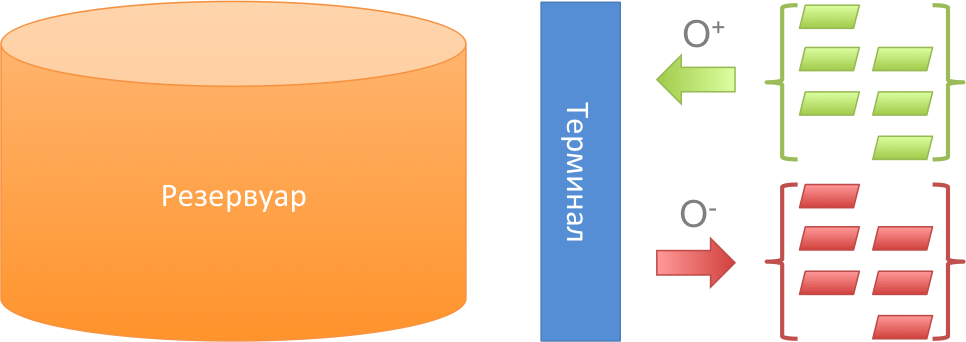
\includegraphics[width=0.6\textwidth]{article-1}
\caption{Рис.~1: Математическая модель.}
\end{figure*}

Заполнение резервуара в момент времени $t$ будем характеризовать переменной $V(t)$ с известным начальным значением $V(0)$. Обслуживание объекта $o_i$ из подпотока $O^+$ может быть начато при наличии в резервуаре достаточного свободного объема; в результате реализации обслуживания такого объекта заполнение резервуара увеличивается на величину $v_i$. Объект $o_i$ из подпотока $O^-$ может быть начат обслуживанием при наличии достаточного заполнения резервуара; в результате реализации его обслуживания заполнение резервуара уменьшается на величину $v_i$. При этом, процессор может обслуживать не более одного объекта каждого из подпотоков одновременно; обслуживание каждого объекта осуществляется без прерываний.

Расписание обслуживания потока $O_n$ определяем как перестановку\\$\rho = {i(1),i(2),…,i(n)}$ совокупности индексов $N = {1,2,…,n}$; при его реализации объект с индексом $i(k)$ обслуживается $k-m$ по очереди ($k=\overline{1,n}$). Расписание $\rho$ именуем допустимым, если в процессе его выполнения удовлетворяются отмеченные выше объемные ограничения, т.е.

\begin{equation*}
0\leq{V(0)} + \sum_{p=1}^{n} v_{i(p)}\leq{V^*}, q=1,2,…,n \eqno{(1)}
\end{equation*}

Совокупность допустимых в модели $M$ расписаний обслуживания обозначим $\Omega$.

Как очевидно, заполнение резервуара после завершения обслуживания всех объектов потока $O_n$ оказывается равным $V(0) + \sum_{i=1}^{n} v_{i(p)}$. При этом выполнение неравенства

\begin{equation*}
0\leq{V(0)} + \sum_{i=1}^{n} v_i\leq{V^*} \eqno{(2)}
\end{equation*}

является необходимым, но недостаточным условием непустоты множества $\Omega$. Приведем иллюстрирующий пример: положим $V(0)=V^*= 5$; подпоток $O^+$ составляет единственный объект с объемной характеристикой, равной 5; в подпоток $O^?$ входит пять объектов, объемная характеристика каждого из них равна 2. Здесь условие (1) выполнено, но допустимого расписания обслуживания не имеется.

Выделим и назовем моделью $M_0$ частый случай модели $M$, в котором все подлежащие обслуживанию объекты изначально присутствуют в системе: $t_k=0$, $k=1,2,…,n$.

% 1. Рассматривается детерминированный поток $O_n=\{o_1, o_2, ... ,o_n\}$ объектов, подлежащих однофазному обслуживанию стационарным процессором $P$. Процессор оснащен двумя независимыми накопительно"=расходными компонентами (резервуарами): компонент $Q_1$ предназначен для временного хранения жидкого продукта ${\textit{П}_1}$, компонент $Q_2$ предназначен для временного хранения жидкого продукта ${\textit{П}_2}$. Нормативный объем компонента $Q_1$ равен $V_1^*$, в начальный момент времени $t = 0$ заполнение $Q_1$ равно $V_1(0)$. Нормативный объем компонента $Q_2$ равен $V_2^*$, в начальный момент времени заполнение $Q_2$ равно $V_2(0)$.

% Для каждого объекта $o_i$, $i=\overline{1,n}$ определены целочисленные параметры: $t_i$ --- момент поступления в очередь на обслуживание, $\tau_i$ --- норма длительности обслуживания, $a_i$ --- штраф за единицу времени пребывания в системе обслуживания, $d_i$ --- мягкий директивный срок завершения обслуживания $(d_i\geq{t_i}+\tau_i)$, $v_i$ --- объемная характеристика. Объекты пронумерованы в порядке их поступления в очередь на обслуживание, т.е. $0\leq{t_1}\leq{…}\leq{t_n}$. Поток $O_n$ можно считать состоящим из четырех независимых подпотоков $O_1^+$, $O_1^-$, $O_2^+$, $O_2^-$, подлежащих обслуживанию процессором $P$. Объекты подпотока $O_1^+$ загружены продуктом ${\textit{П}_1}$, который при обслуживании процессором $P$ должен быть перемещен в компонент $Q_1$; объекты подпотока $O_2^+$ загружены продуктом ${\textit{П}_2}$, который при обслуживании процессором $P$ должен быть перемещен в компонент $Q_2$; объекты подпотоков $O_1^-$ и $O_2^-$ поступают для обслуживания порожними и процессор $P$ обеспечивает их загрузку соответственно продуктом ${\textit{П}_1}$, и ${\textit{П}_2}$ путем перекачки из компонентов $Q_1$ и $Q_2$. Подпотоки $O_1^+$, $O_1^-$, $O_2^+$, $O_2^-$ удовлетворяют условию $O_1^+\cup{O_1^-}\cup{O_2^+}\cup{O_2^-}=O_n$ и попарно не пересекаются. Принадлежность объекта $o_i$ тому или иному подпотоку характеризуется параметром $w_i$: $w_i=+1$, если $o_i\in{O_1^+}$; $w_i=-1$, если $o_i\in{O_1^-}$; $w_i=+2$, если $o_i\in{O_2^+}$; $w_i=-2$, если $o_i\in{O_2^-}$.

% В результате обслуживания очередного объекта $o_i$ из подпотока $O_1^+$ ($O_2^+$) заполнение соответствующего компонента $Q_1$ ($Q_2$) увеличивается на величину $v_i$. По завершению обслуживания очередного объекта $o_i$ из подпотока $O_1^-$ ($O_2^-$) заполнение соответствующего компонента $Q_1$ ($Q_2$) уменьшается на величину $v_i$. Обслуживание очередного объекта из подпотока $O_1^+$ ($O_2^+$) может начаться при наличии достаточного свободного объема в соответствующем компоненте $Q_1$ ($Q_2$). Объект подпотока $O_1^-$ ($O_2^-$) может быть принят процессором $P$ на обслуживание при наличии достаточного количества продукта в $Q_1$ ($Q_2$). Обслуживание каждого объекта осуществляется без прерываний; необслуженный объект не может покинуть очередь; непроизводительные простои процессора не предусмотрены; одновременное обслуживание процессором двух и более объектов запрещено. Стратегия $S$ обслуживания объектов потока $O_n$ представляет собой произвольную перестановку $S=\{i_1, i_2, … ,i_n\}$ совокупности индексов $N=\{1, 2, … ,n\}$; при её реализации объект с индексом $i_k$ обслуживается $k$-м по очереди, $k=\overline{1,n}$. Стратегию $S$ именуем допустимой, если удовлетворяются отмеченные выше объемные ограничения на обслуживание объектов $o_i$, $i=\overline{1,n}$. Обозначим через $\Omega$ множество допустимых стратегий. Очевидно, что необходимыми условиями непустоты множества $\Omega$ является выполнение неравенств:

% \[0\leq{V_1(0)}+\sum_{i:\{w_i=\{+1,-1\}\}} sign(w_i)\*v_i\leq{V_1^*},\]
% \[0\leq{V_2(0)}+\sum_{i:\{w_i=\{+2,-2\}\}} sign(w_i)\*v_i\leq{V_2^*}.\]

% Для известной стратегии $S$ арифметически вычисляются обозначаемые через $t^*(i(k), S)$ и $t^{**}(i(k), S)$ соответственно значения моментов начала и завершения обслуживания каждого объекта с индексом $i(k)$, $i=\overline{1,n}$.

% 2. На практике качество стратегии $S$ в зависимости от складывающейся эксплуатационной ситуации оценивается по значению критерия $K_1(S)$ или $K_2(S)$. При этом критерий $K_1(S)$ представляет собой суммарный штраф по объектам потока $O_n$ за время пребывания в системе обслуживания; критерий $K_2(S)$ оценивает максимальное по продолжительности нарушение директивного срока завершения обслуживания среди всех объектов потока $O_n$. С учетом введенных выше обозначений, вводимые критерии определяются следующим образом:

% \[K_1(S)=\sum_{k=1}^n a_{i(k)}(t^*(i(k),S)-t_{i(k)}),\]
% \[K_{ 2 }(S)=\underset {1\leq{k}\leq{n}}{max} (t^{ ** }(i(k),S)-d_{ i(k) },0).\]

% Изучаемые в данной работе однокритериальные задачи записываются в виде:

% \[\underset{S\in\Omega}{min}~K_1(S),\]
% \[\underset{S\in\Omega}{min}~K_2(S).\]

% Обе задачи относятся к числу NP-трудных~[2]. Для их решения в работе разрабатываются алгоритмы, основанные на концепции дискретного динамического программирования~[3,\,4,\,5].

% Работа выполнена при поддержке РФФИ (проект \hbox{№\,15-07-03141}).

% \begin{ptkreferences}
% \item
% Северный завоз~/ Материал из Википедии – свободной энциклопедии. URL~: http://ru.wikipedia.org/wiki/Северный\_завоз (дата обращения~: 10.03.17).
% \item
% Гэри~М., Джонсон~Д. Вычислительные машины и труднорешаемые задачи. --- М.~: Мир, 1982. --- 416\,с.
% \item
% Коган~Д.\,И., Куимова~А.\,С., Федосенко~Ю.\,С. Задачи обслуживания бинарного потока объектов в системе с накопительно"=расходным компонентом~// Автоматика и телемеханика. --- 2014. №\,7. --- С.\,122--135.
% \item
% Беллман~Р., Дрейфус~С. Прикладные задачи динамического программирования. --- М.~: Наука, 1965. --- 457\,с.
% \item
% Коган~Д.\,И., Федосенко~Ю.\,С. Общая схема реализации алгоритмов динамического программирования в задачах синтеза стратегий однопроцессорного обслуживания потока объектов~// Сб. <<Информатика и технологии. Инновационные технологии в промышленности и информатике>>. --- М.~: МИРЭА, --- 2016. С.\,154--157.
% \end{ptkreferences}
\end{ptkarticle}
\end{document}
